\documentclass[t]{beamer}
% \documentclass[handout,xcolor=pdftex,dvipsnames,table]{beamer}

\mode<presentation>
{
  \usetheme{Warsaw}
  \usecolortheme{whale}
  % or ...

  % or whatever (possibly just delete it)
  \setbeamertemplate{navigation symbols}{}
}

\usepackage{hyperref}
\usepackage{media9}

% make a command to decrease font size locally when desired
\newcommand\Fontvi{\fontsize{8.5}{7.2}\selectfont}



\setbeamertemplate{itemize items}[ball]
\setbeamertemplate{itemize subitem}[triangle]
\setbeamertemplate{itemize subsubitem}[circle]
\setbeamercovered{invisible}

\usepackage{palatino} 
\usepackage{listings} % Gives syntax highlighting for python code. 
\usepackage{color} % Used for syntax highlighting. 
\usepackage{textcomp} % Used for syntax highlighting. 
\usepackage{caption}
\captionsetup{labelformat=empty,labelsep=none}
% This gives syntax highlighting in the python environment 
\definecolor{gray}{gray}{0.5} 
\definecolor{key}{rgb}{0,0.5,0} 
\lstset{
language=python,
basicstyle=\ttfamily\tiny, 
otherkeywords={1, 2, 3, 4, 5, 6, 7, 8 ,9 , 0, -, =, +, [, ], (, ), \{, \}, :, *, !}, 
keywordstyle=\color{blue}, 
stringstyle=\color{red},
showstringspaces=false,
alsoletter={1234567890},
otherkeywords={\ , \}, \{},
keywordstyle=\color{blue},
emph={access,and,break,class,continue,def,del,elif ,else,%
except,exec,finally,for,from,global,if,import,in,is,%
lambda,not,or,pass,print,raise,return,try,while},
emphstyle=\color{black}\bfseries,
emph={[2]True, False, None, self},
emphstyle=[2]\color{green},
emph={[3]from, import, as},
emphstyle=[3]\color{blue},
upquote=true,
morecomment=[s]{"""}{"""},
commentstyle=\color{gray}\slshape,
emph={[4]1, 2, 3, 4, 5, 6, 7, 8, 9, 0},
emphstyle=[4]\color{blue},
literate=*{:}{{\textcolor{blue}:}}{1}%
{=}{{\textcolor{blue}=}}{1}%
{-}{{\textcolor{blue}-}}{1}%
{+}{{\textcolor{blue}+}}{1}%
{*}{{\textcolor{blue}*}}{1}%
{!}{{\textcolor{blue}!}}{1}%
{(}{{\textcolor{blue}(}}{1}%
{)}{{\textcolor{blue})}}{1}%
{[}{{\textcolor{blue}[}}{1}%
{]}{{\textcolor{blue}]}}{1}%
{<}{{\textcolor{blue}<}}{1}%
{>}{{\textcolor{blue}>}}{1},%
numbers=none,
}

\newcommand{\putat}[3]{\begin{picture}(0,0)(0,0)\put(#1,#2){#3}\end{picture}}



\title[]{Python Workshop\\
 
\includegraphics[scale=0.055]{figures/python-app.png}\hspace{5 pt}How we use python\hspace{5 pt}
\includegraphics[scale=0.055]{figures/python-app.png} }

\author[Hughes] % (optional, use only with lots of authors)
{Joseph D.~Hughes}
\institute[USGS] % (optional, but mostly needed)
{
  U.S. Geological Survey\\
  Florida Water Science Center, Tampa, Florida USA
  }
  \titlegraphic{
\includegraphics[scale=0.5]{figures/c_USGSid1.pdf}}
  

\date[UQ12] % (optional, should be abbreviation of conference name)
{USGS National Groundwater Workshop, August 2012}

\subject{Python}


\begin{document}

\begin{frame}
  \titlepage
\end{frame}
\logo{\vspace{-0.3cm} 
\includegraphics[width=1.5cm]{figures/c_USGSid1.pdf}\hspace*{11.10cm}}  

%\begin{frame}{How we use python}
%\tableofcontents
%\end{frame}

\section{Creating input files}
\subsection{From raw data}
\begin{frame}{Create GHB file from raw data (1)}
  \tiny{[xoff,yoff,rot]=[1000,1000,45]}
  \begin{figure}[ht]
  \centering
         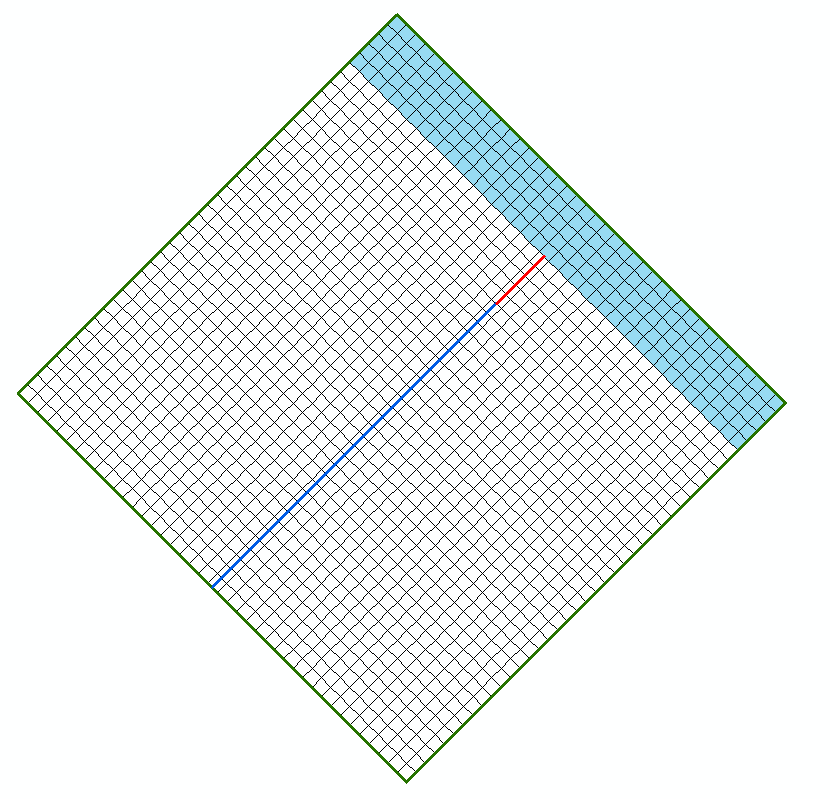
\includegraphics[height=0.8\textheight]{figures/CoastalModelBoundary.png}
   \end{figure}
\end{frame}

\begin{frame}{Create GHB file from raw data (2)}
  \small{\texttt{CreateCoastalGHB.py}}
  \begin{figure}[ht]
  \centering
        \lstset{numbers=left}
        \lstinputlisting[language=python, firstline=1,lastline=18,firstnumber=1]{python/CreateCoastalGHB.py}
   \end{figure}
\end{frame}

\begin{frame}{Create GHB file from raw data (3)}
  \small{\texttt{CreateCoastalGHB.py}}
  \begin{figure}[ht]
  \centering
        \lstset{numbers=left}
        \lstinputlisting[language=python, firstline=19,lastline=41,firstnumber=19]{python/CreateCoastalGHB.py}
   \end{figure}
\end{frame}

\begin{frame}{Output GHB file from raw data (4)}
  \small{\texttt{Model.ghb}}
  \begin{figure}[ht]
  \centering
        \lstset{numbers=left}
        \lstinputlisting[ firstline=1,lastline=13,firstnumber=1]{data/Model.ghb}
        \lstinputlisting[ firstline=204,lastline=210,firstnumber=210]{data/Model.ghb}
   \end{figure}
\end{frame}

\subsection{From model results}
\begin{frame}{Extract heads to create a new initial head array}
\small{\texttt{extractSteadyHead.py}}
  \begin{figure}[ht]
  \centering
        \lstset{numbers=left}
        \lstinputlisting[language=python, firstline=1,lastline=18,firstnumber=1]{python/extractSteadyHead.py}
   \end{figure}
\end{frame}

\section{Processing output files}
\subsection{Reading binary head file}
\begin{frame}{Binary head data}
\small{\texttt{plotHeads.py}}
  \begin{figure}[ht]
  \centering
        \lstset{numbers=left}
        \lstinputlisting[language=python, firstline=43,lastline=49,firstnumber=43]{python/plotHeads.py}
        \lstinputlisting[language=python, firstline=55,lastline=63,firstnumber=55]{python/plotHeads.py}
   \end{figure}
\end{frame}

\section{Making figures and animations}
\subsection{Using matplotlib}
\begin{frame}{Figures (1)}
\small{\texttt{plotHeads.py}}
  \begin{figure}[ht]
  \centering
        \lstset{numbers=left}
        \lstinputlisting[language=python, firstline=84,lastline=92,firstnumber=84]{python/plotHeads.py}
   \end{figure}
\end{frame}

\begin{frame}{Figures (2)}
  \begin{figure}[ht]
  \centering
       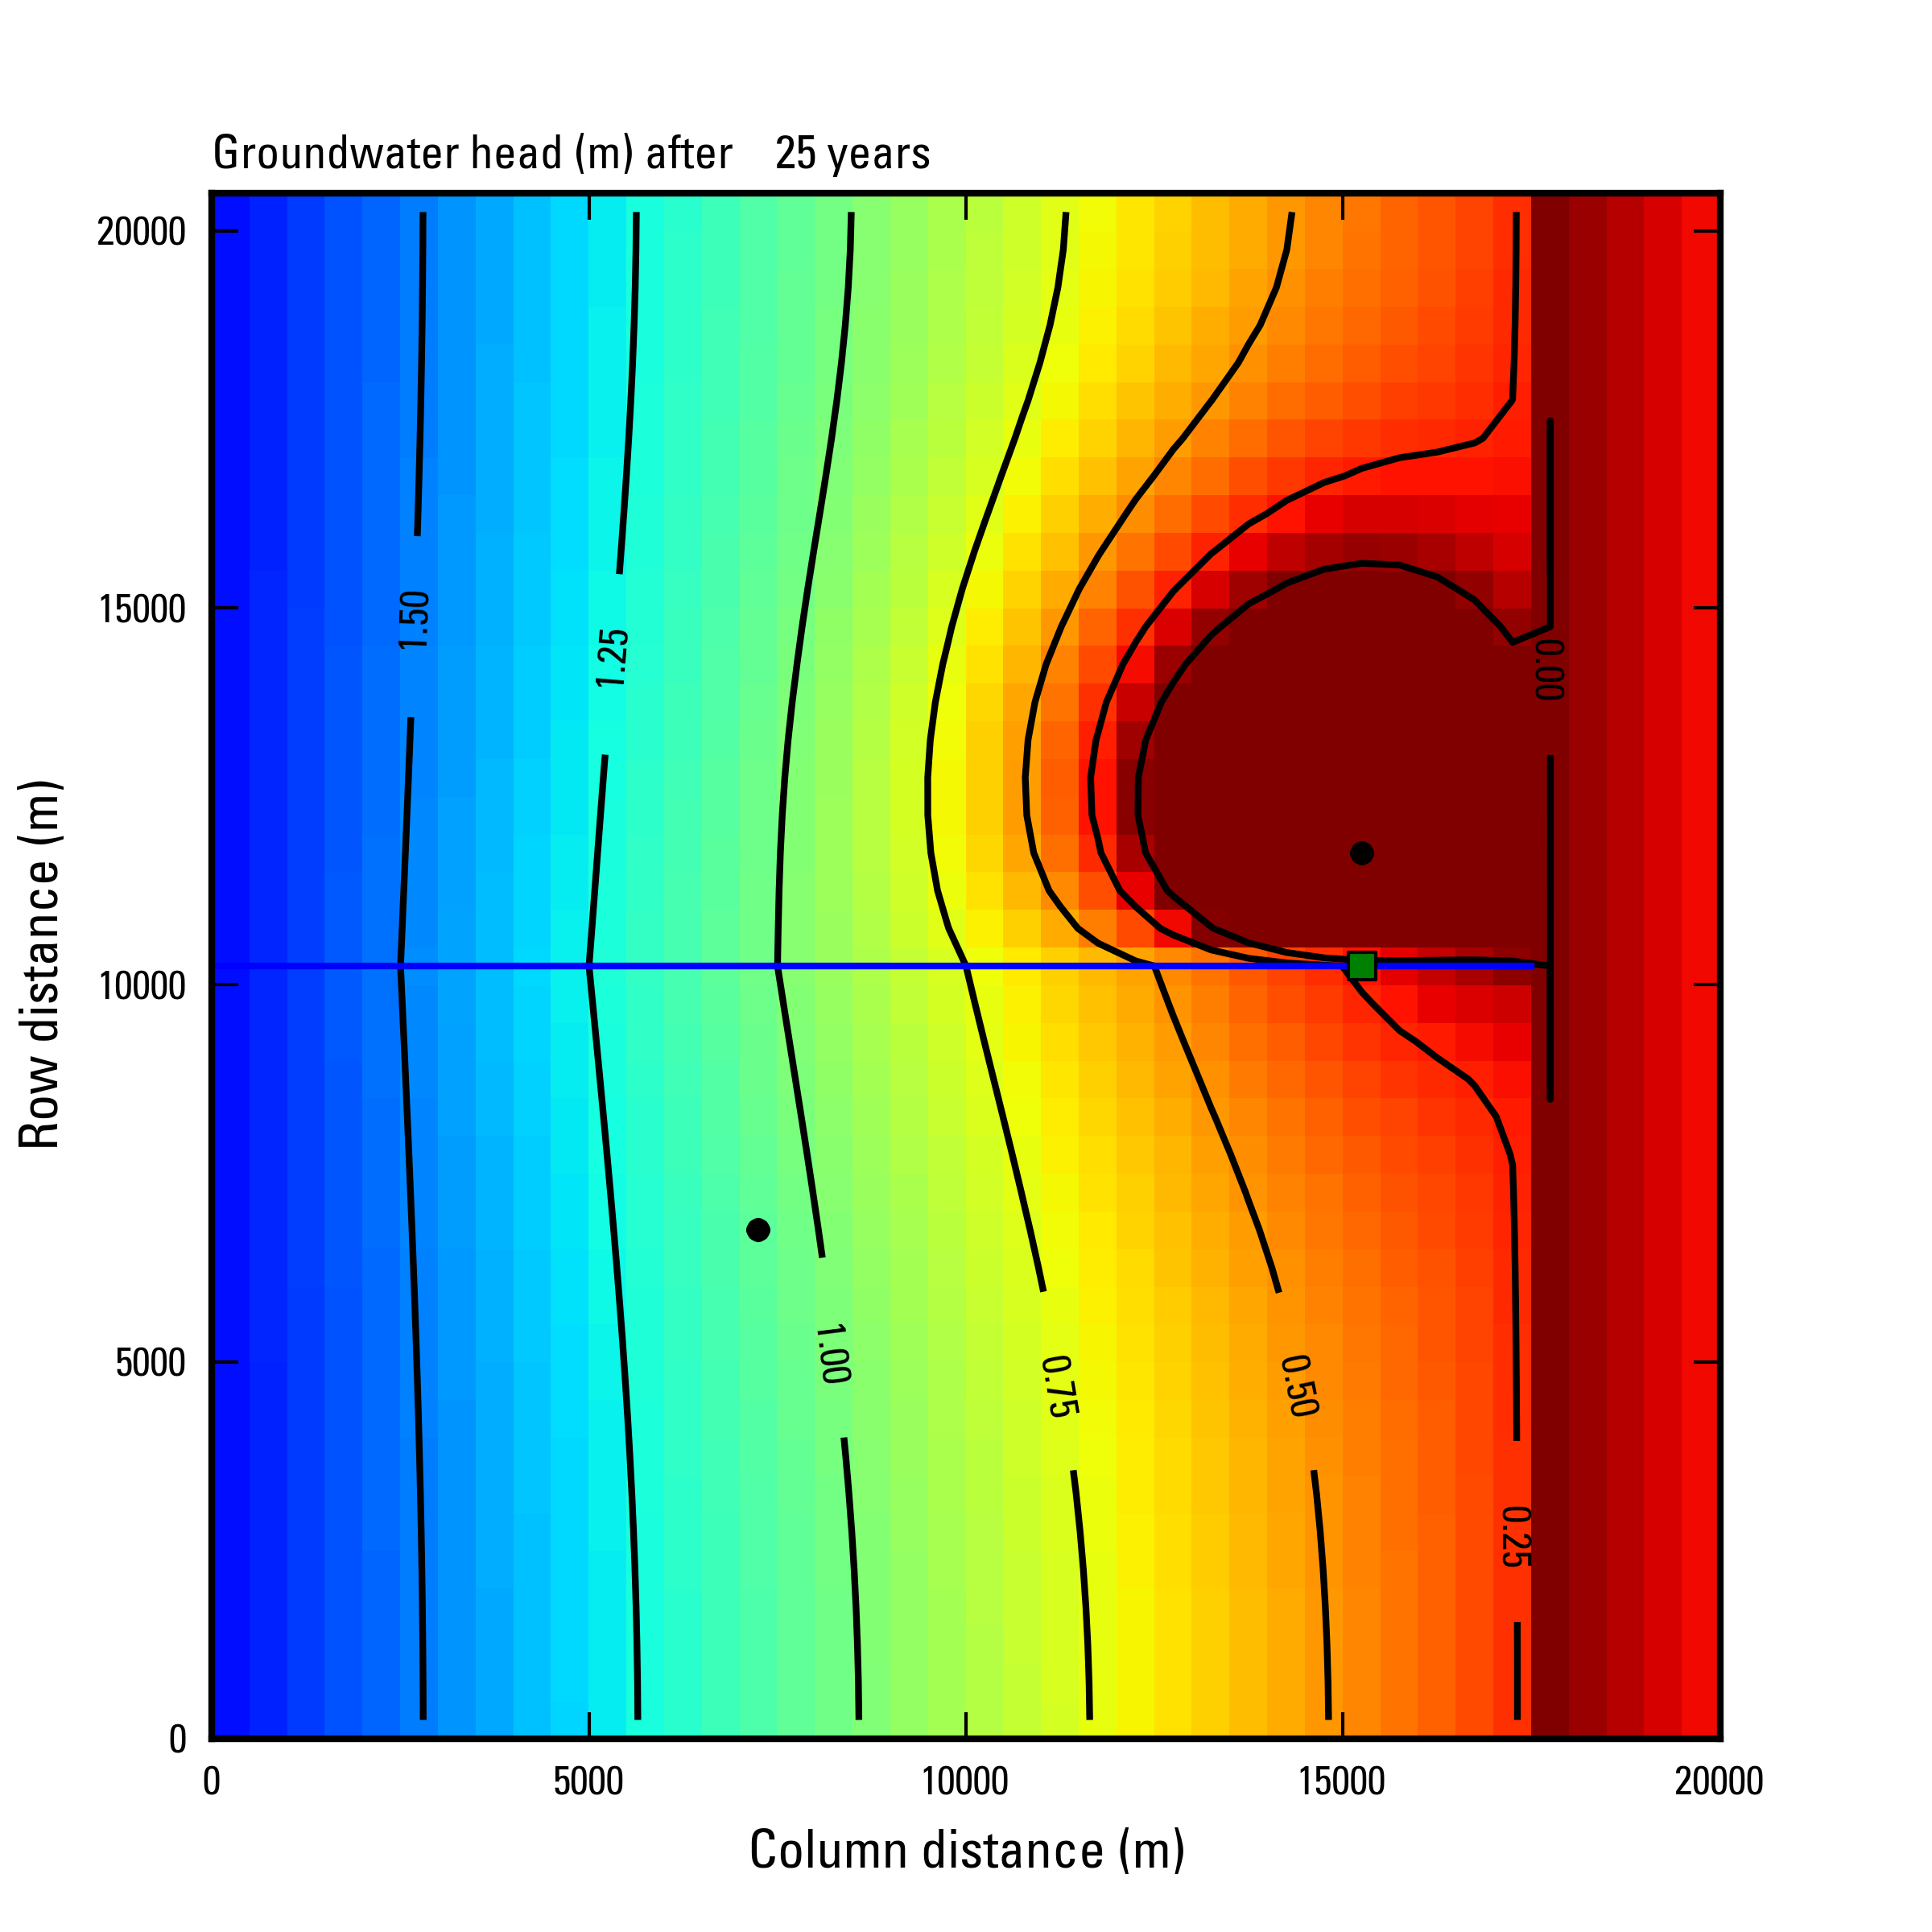
\includegraphics[width=0.5\textwidth]{figures/MF_Results_00024.png} 
       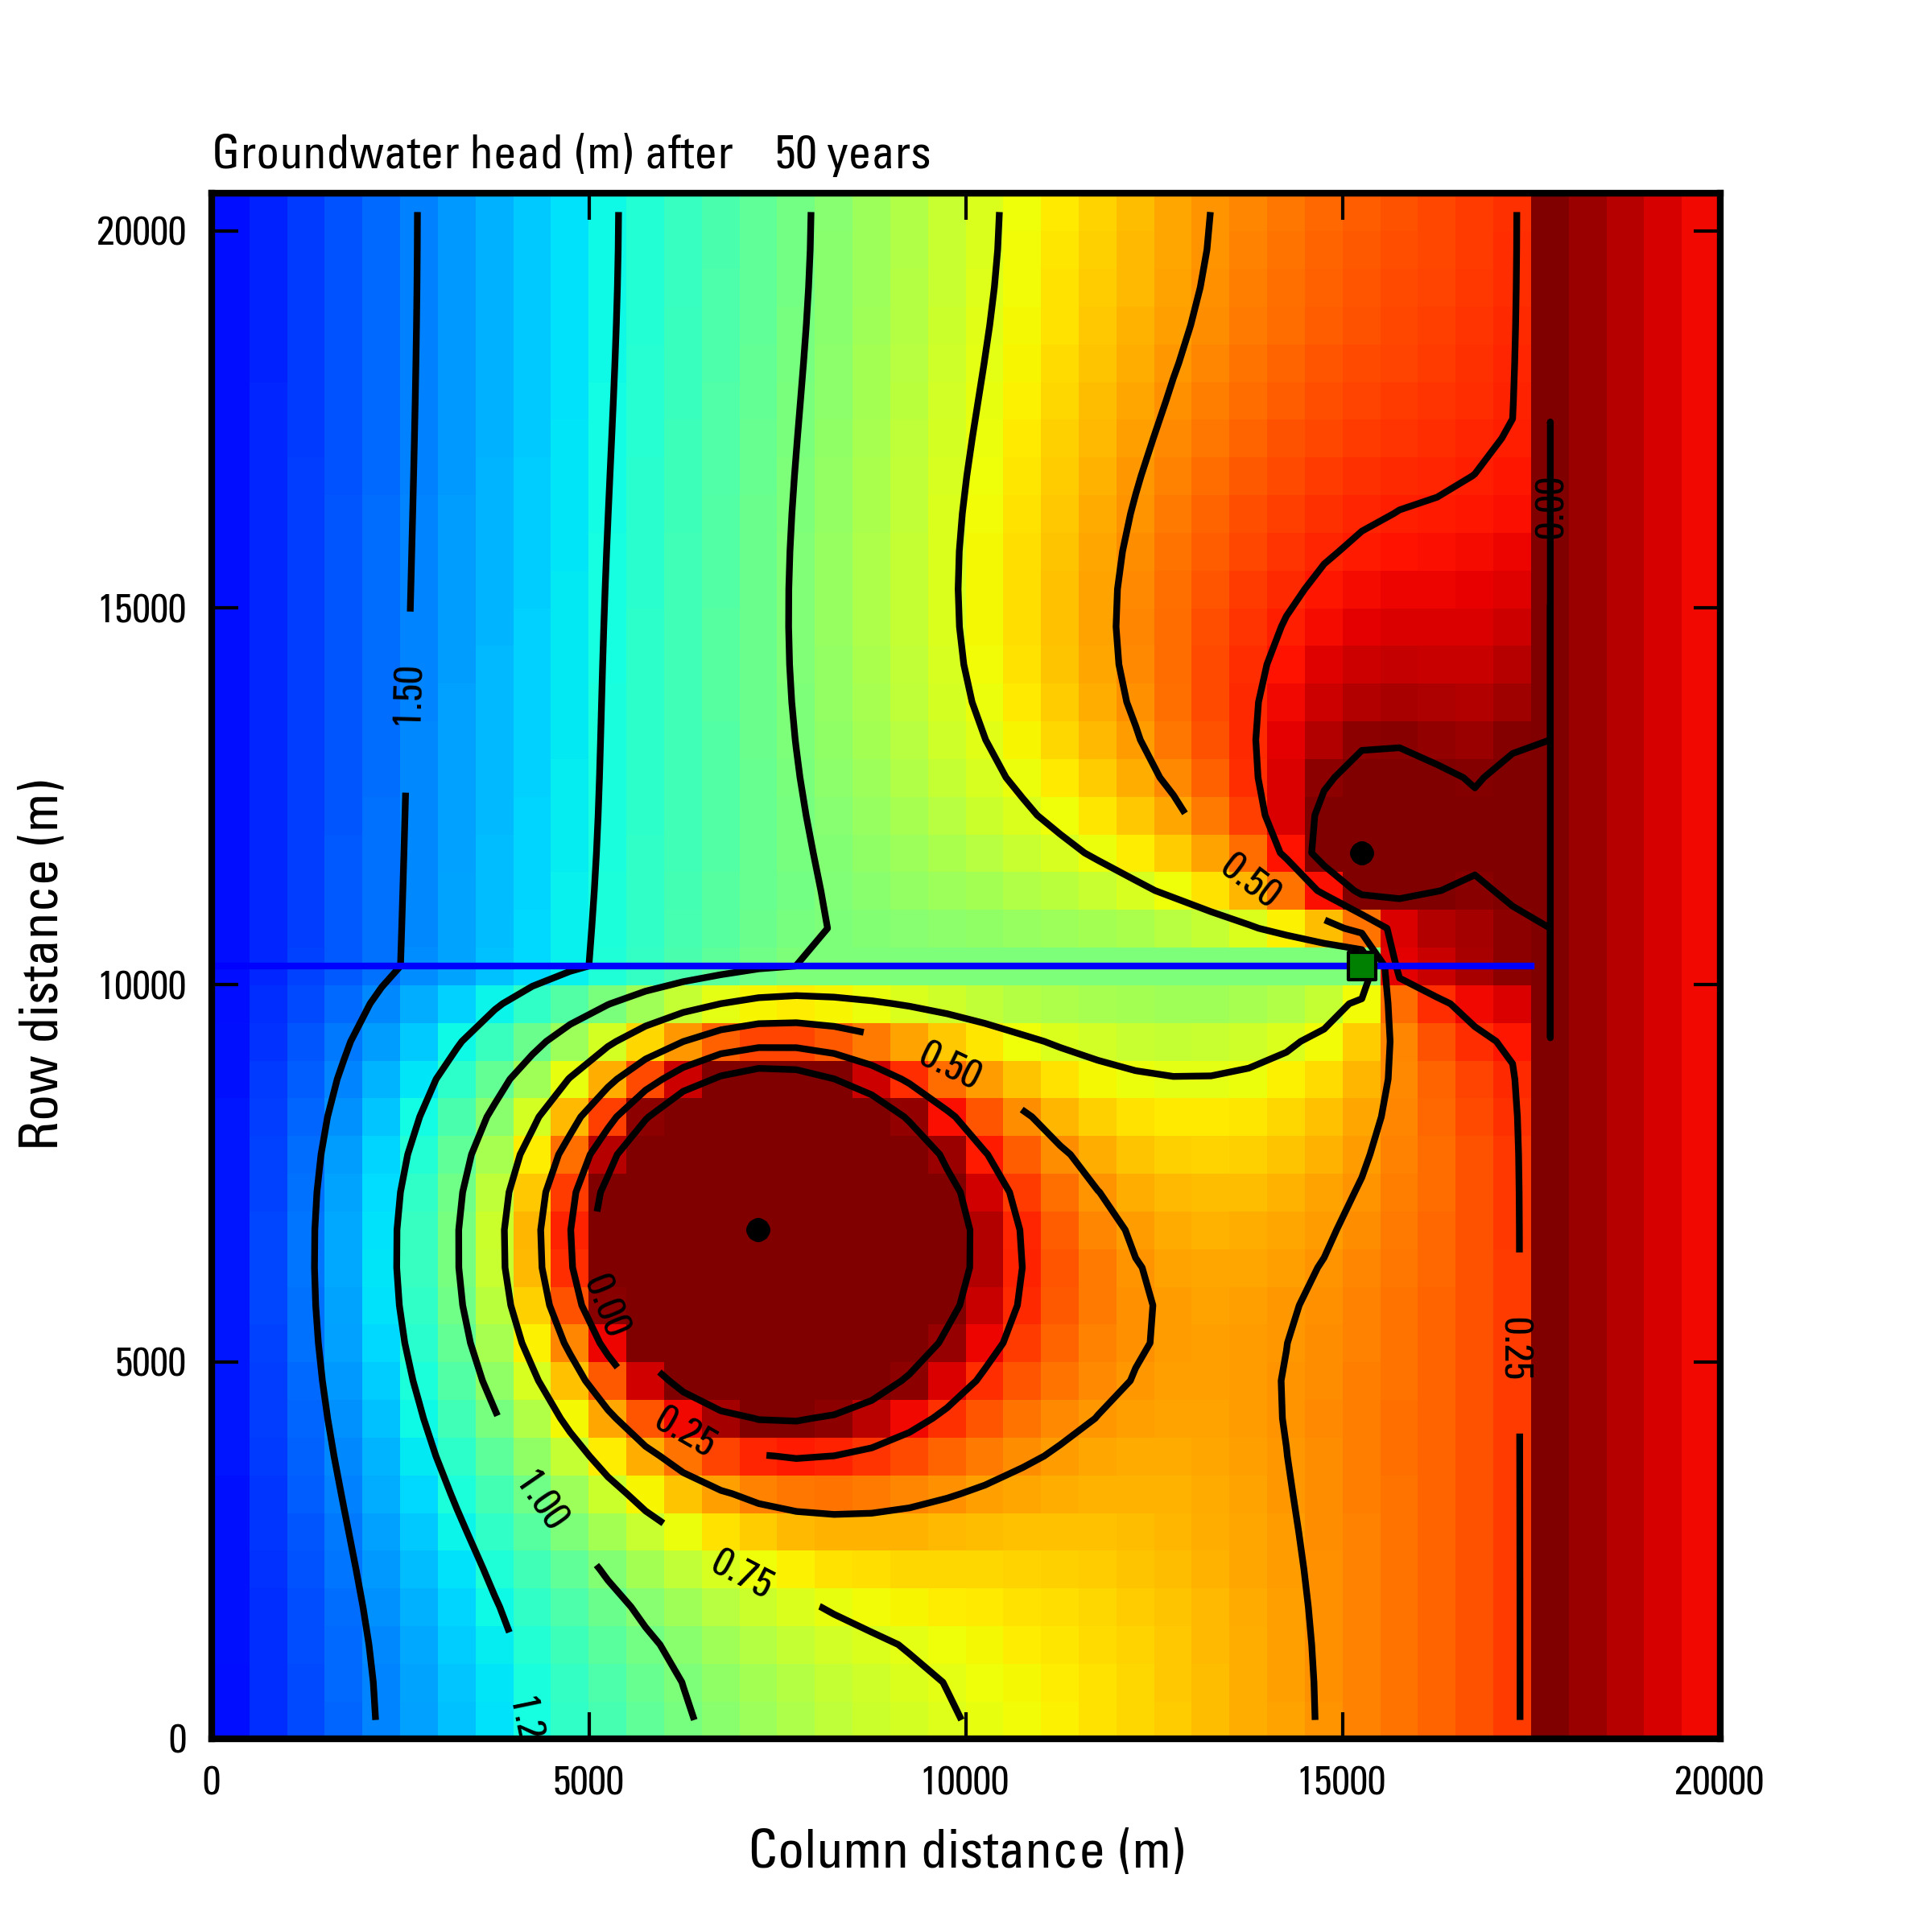
\includegraphics[width=0.5\textwidth]{figures/MF_Results_00049.png}
   \end{figure}
\end{frame}


\subsection{Animations}
\begin{frame}{Using \texttt{ffmpeg.exe}}
  \begin{figure}[ht]
  \centering
        \lstset{numbers=left}
        \lstinputlisting[language=python, firstline=101,lastline=108,firstnumber=101]{python/plotHeads.py}
   \end{figure}
\end{frame}

\begin{frame}{Using \texttt{ffmpeg.exe}}
\begin{center}
\includemedia[
activate=onclick,width=0.8\textheight]{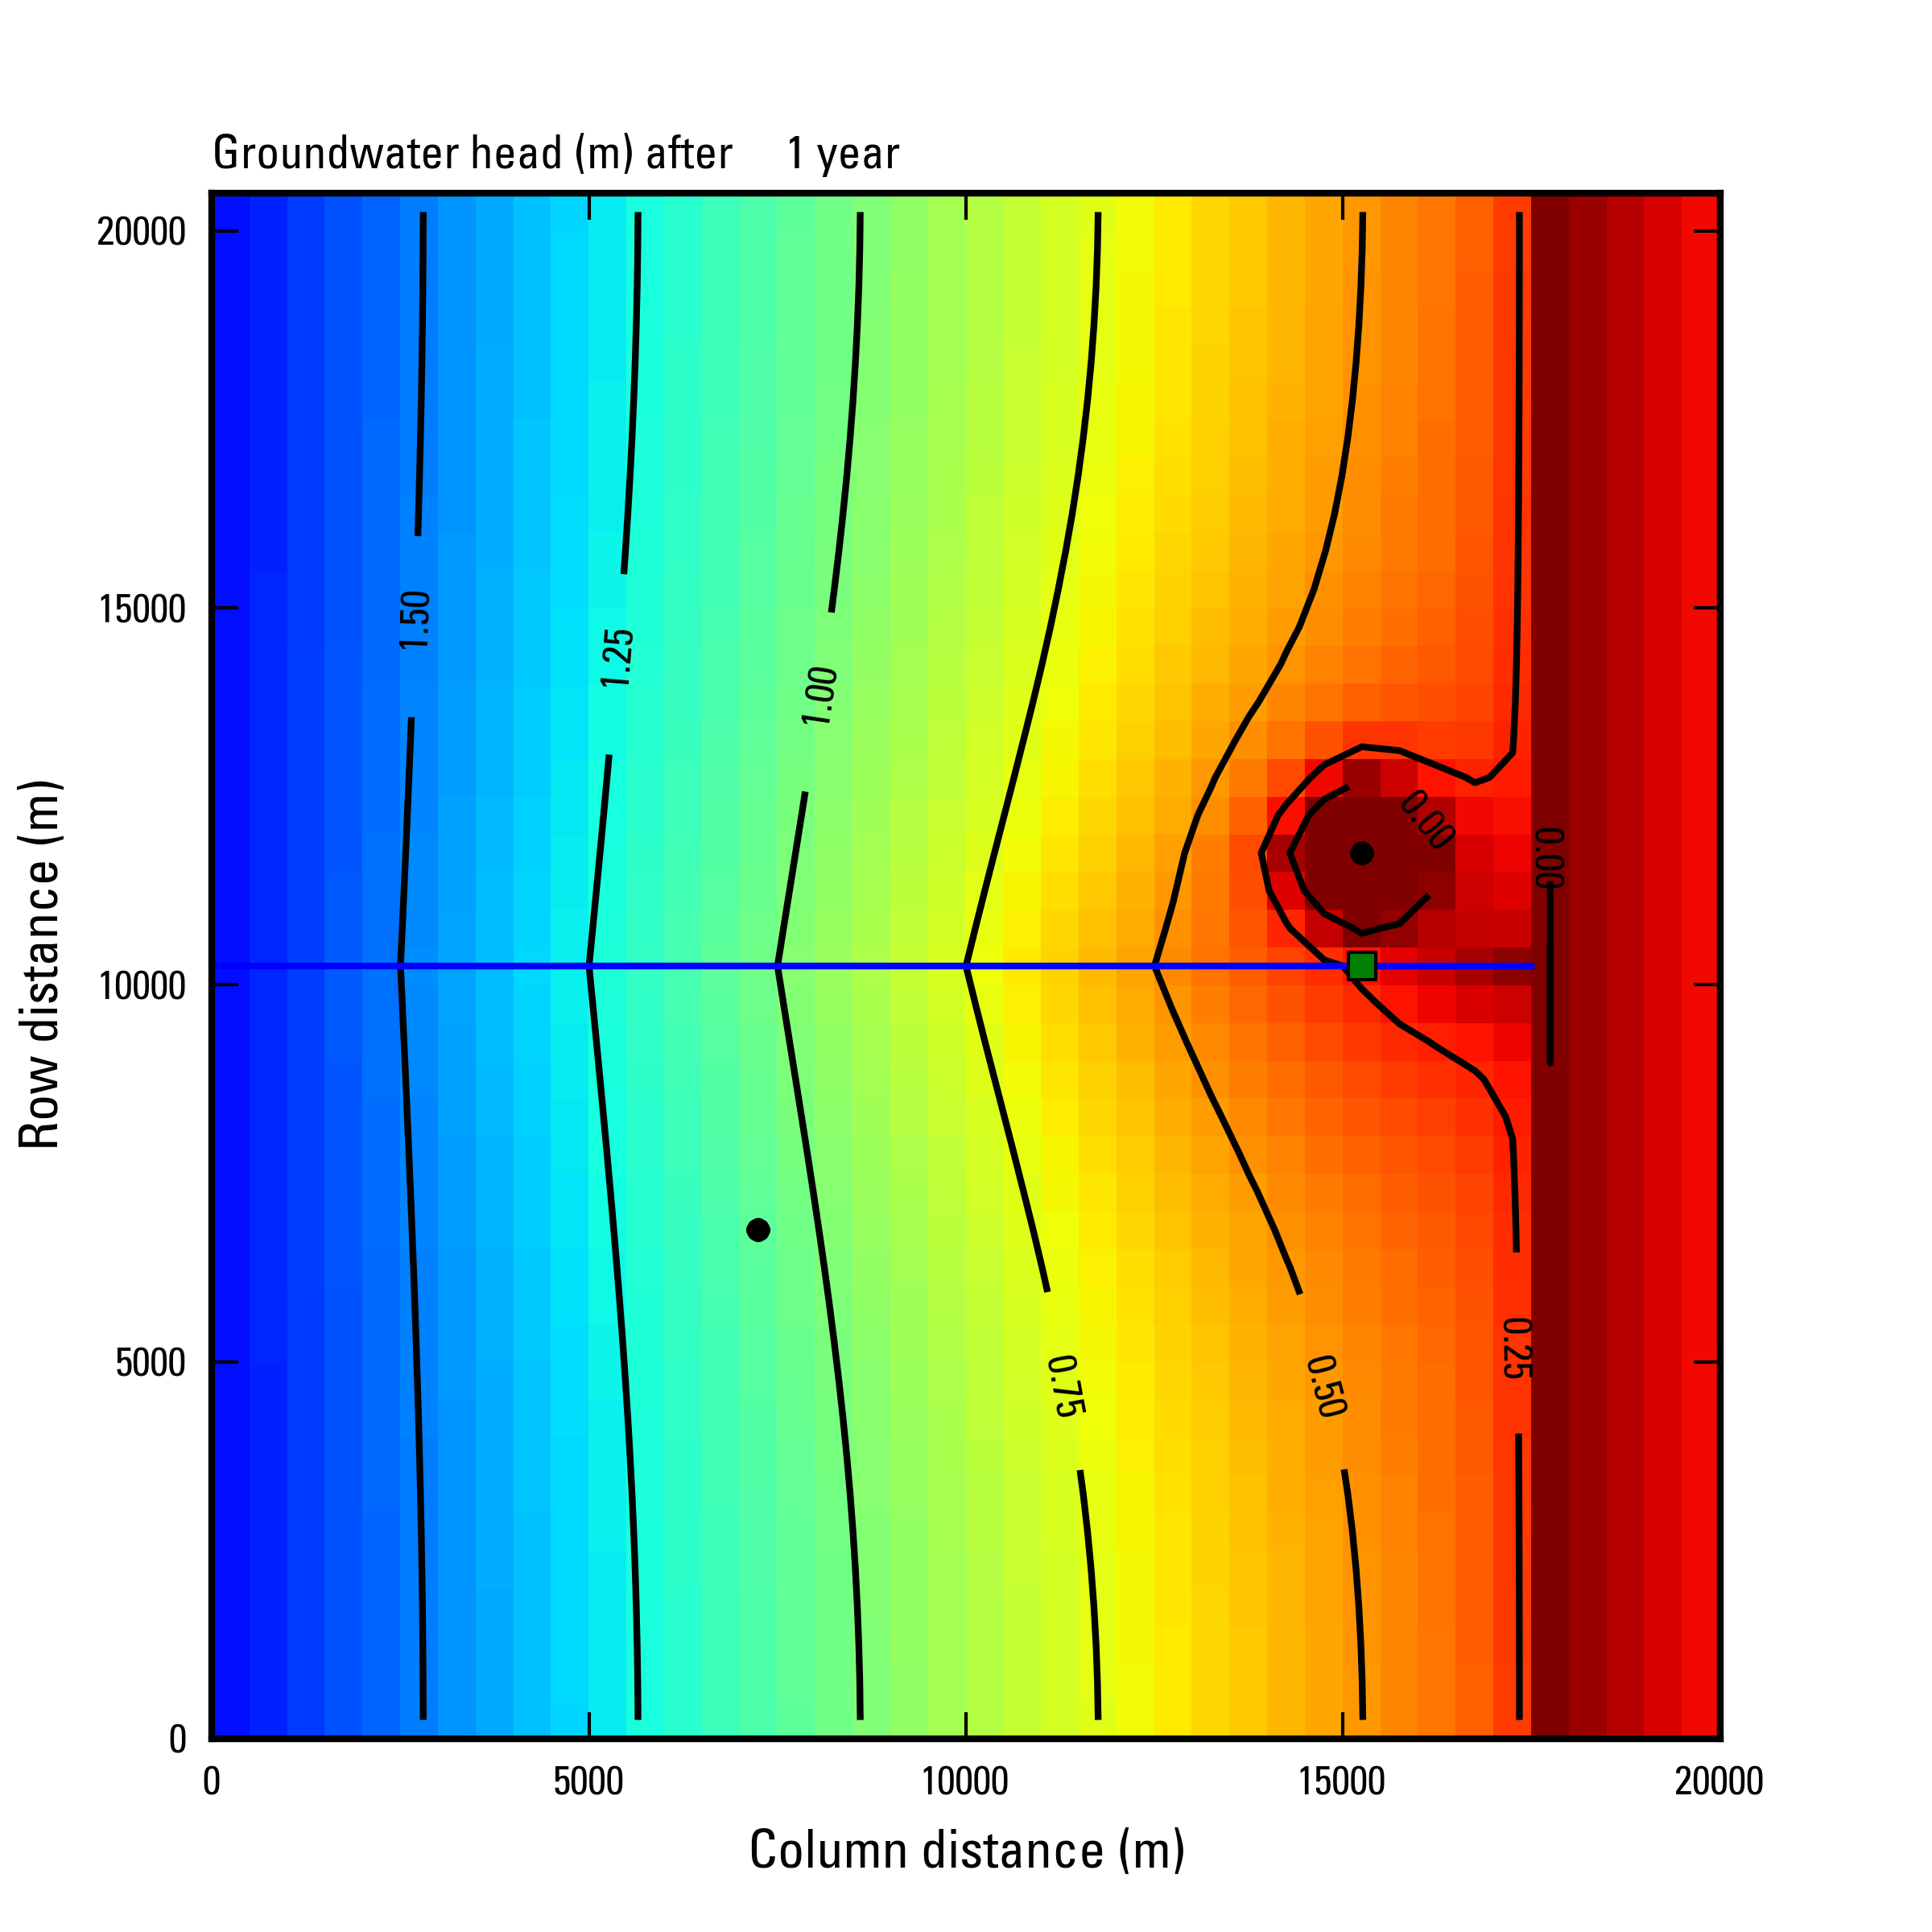
\includegraphics[height=0.8\textheight]{figures/MF_Results_00000.png}}{figures/MF_Results.swf}
\end{center}
\end{frame}

\section{Making shapefiles}
\subsection{Get data from MODFLOW file}
\begin{frame}{Making shapefiles (1)}
\small{\texttt{makeShapefileFromDIS.py}}
  \begin{figure}[ht]
  \centering
        \lstset{numbers=left}
        \lstinputlisting[language=python, firstline=4,lastline=6,firstnumber=4]{python/makeShapefileFromDIS.py}
        \lstinputlisting[language=python, firstline=89,lastline=103,firstnumber=89]{python/makeShapefileFromDIS.py}
   \end{figure}
\end{frame}

\subsection{Make shapefile}
\begin{frame}{Making shapefiles (2)}
\small{\texttt{makeShapefileFromDIS.py}}
  \begin{figure}[ht]
  \centering
        \lstset{numbers=left}
        \lstinputlisting[language=python, firstline=104,lastline=123,firstnumber=104]{python/makeShapefileFromDIS.py}
   \end{figure}
\end{frame}

\begin{frame}{Making shapefiles (3)}
\small{\texttt{makeShapefileFromDIS.py}}
  \begin{figure}[ht]
  \centering
        \lstset{numbers=left}
        \lstinputlisting[language=python, firstline=124,lastline=135,firstnumber=124]{python/makeShapefileFromDIS.py}
   \end{figure}
\end{frame}

\end{document}